\documentclass[conference]{IEEEtran}

\usepackage{graphicx}
\usepackage{hyperref}
\usepackage{xspace}
\usepackage{listings}
\usepackage[usenames, dvipsnames]{color}

\lstset{language=Python}

\lstdefinestyle{custompython}{
	belowcaptionskip=1\baselineskip,
	frame=lr,
	xleftmargin=\parindent,
	language=Python,
	basicstyle=\footnotesize\ttfamily,
	keywordstyle=\bfseries\color{MidnightBlue},
	stringstyle=\color{PineGreen},
  commentstyle=\color{Magenta}
}
         

\graphicspath{{./img/}}

\hyphenation{op-tical net-works semi-conduc-tor}


\lstset{language=Python}

\definecolor{LightGray}{RGB}{250,250,250}

\lstdefinestyle{custompython}{
	captionpos=b,                    % sets the caption-position to bottom
	% frame=tb,
	xleftmargin=\parindent,
	language=Python,
	basicstyle=\footnotesize\ttfamily,
	keywordstyle=\bfseries\color{MidnightBlue},
	stringstyle=\color{PineGreen},
  	commentstyle=\color{Magenta},
  	backgroundcolor=\color{LightGray}
}


\newcommand{\tool}{Flask Dashboard\xspace}
\newcommand{\zee}{Zeeguu\xspace}
\newcommand{\git}{\texttt{git}\xspace}
\newcommand{\install}{{\small \texttt{pip install flask\_dashboard}}\xspace}
\newcommand{\activeUserCount}{two hundred\xspace}
\newcommand{\code}[1]{\texttt{#1}\xspace}
\newcommand{\perspective}[1]{{\small {\texttt{#1}}\xspace}}

\usepackage{fourier-orns}

\definecolor{myred}{RGB}{230, 20, 70}
\definecolor{mygreen}{RGB}{60, 180, 75}


\newcommand{\niceseparator}
	{
		\begin{center}
  		% $\ast$~$\ast$~$\ast$
  		% $\clubsuit$~$\clubsuit$~$\clubsuit$
  		\leafleft
		\end{center}
	}

% Endpoint Names 
%\newcommand{\epDecoration}[1]{{\small {\bf #1}}\xspace}
\newcommand{\epDecoration}[1]{\code{#1}}

\newcommand{\epTranslations}{{\color{myred} \epDecoration{api.get\_possible\_translations}}\xspace}
\newcommand{\epOutcome}{\epDecoration{api.report\_exercise\_outcome}}
\newcommand{\epFeedItems}{\epDecoration{api.get\_article\_difficulties}}



% Author Comments / Discussion

\definecolor{mlcolor}{RGB}{140, 140, 205}
\definecolor{vacolor}{RGB}{255, 0, 255}

\newcommand{\ml}[1]{ 
	{\footnotesize \color{mlcolor}ML: #1}
	}

\newcommand{\va}[1]{ 
	{\footnotesize \color{vacolor}VA: #1}
}


\newcommand{\mltp}[1]{\ml{Thijs, Patrick: #1}}
\newcommand{\mlv}[1]{\ml{Vasilios: #1}}

\definecolor{todocolor}{RGB}{200, 140, 160}

\newcommand{\todo}[1]{ 
	{\footnotesize \color{todocolor}Todo: #1}
	}

\newcommand{\Fref}[1]{Fig.~\ref{#1}}
\newcommand{\Sref}[1]{Sec.~\ref{#1}}




\begin{document}
%
\title{Visualizing Evolving Service Performance in Python }
% Alternative Titles: The Importance of Visualization in the Performance Monitoring of Python Web Services


% author names and affiliations
% use a multiple column layout for up to three different
% affiliations
%\author{\IEEEauthorblockN{Michael Shell}
%\IEEEauthorblockA{School of Electrical and\\Computer Engineering\\
%Georgia Institute of Technology\\
%Atlanta, Georgia 30332--0250\\
%Email: http://www.michaelshell.org/contact.html}
%\and
%\IEEEauthorblockN{Homer Simpson}
%\IEEEauthorblockA{Twentieth Century Fox\\
%Springfield, USA\\
%Email: homer@thesimpsons.com}
%\and
%\IEEEauthorblockN{James Kirk\\ and Montgomery Scott}
%\IEEEauthorblockA{Starfleet Academy\\
%San Francisco, California 96678--2391\\
%Telephone: (800) 555--1212\\
%Fax: (888) 555--1212}}

\author{
\IEEEauthorblockN{NAMES ORDER TBA}\\
Johann Bernoulli Institute of Mathematics and Computer Science\\
University of Groningen\\
Groningen, the Netherlands\\
Email: \{v.andrikopoulos,m.f.lungu\}@rug.nl, \{t.klooster.1,p.p.vogel\}@student.rug.nl
}

% make the title area
\maketitle

\begin{abstract}
The abstract goes here.
\end{abstract}

% no keywords

\IEEEpeerreviewmaketitle



\section{Introduction}
Every system is a distributed system nowadays \cite{cavage2013there}. 
% \hfill mds
 
% \hfill August 26, 2015

Python is currently one of the most popular programming languages. At the time of writing this paper\footnote{June 2017} Python is the 4th most popular programming language cf. the Tiobe Index\footnote{TIOBE programming community index is a measure of popularity of programming languages, created and maintained by the TIOBE Company based in Eindhoven, the Netherlands}. 

\todo{Flask summary goes here}

A search on GitHub with the keyword ``language:Python'' returns more than 500K open source projects written in the language. If we restrict the search by adding the keyword ``Flask'' we obtain a listing of 25K projects, that is, 5\% of all the Python projects. Flask -- advertised as a {\em micro-framework} -- is a lightweight alternative to web site and service development. 


However, there is no dedicated solution for monitoring the performance of Flask web-applications. Thus, every one of those Flask projects faces one of the following options when confronted with the need of gathering insight into the runtime behavior of their implemented service: 

  \begin{enumerate}

    \item Use a heaviweight professional API monitoring setup they require setting up a different server \mltp{can we find a few examples of professional but overkill tools? ideally they require setting up a bunch of servers, and writing configs in XML!}. 

    \item Implement their own analytics tool 

    \item Live wihout analytics insight into their services \footnote{This is very real option: and is exactly what happened to the API that will be presented in this case study for many months. }

  \end{enumerate}

\todo{For the first point in the list, we can also argue that analytics solutions like Google Analytics can be used, but they have no notion of versioning/integration with the development lifecycle. Feel free to cite \cite{papazoglou2011managing} for service evolution purposes}

For projects which are done on a budget (e.g. research projects) the first and the second options are often not available due to time and financial constraints. 

To avoid these projects ending up in the third situation, in this paper we present a low-effort, lightweight service monitoring API for Flask and Python web-services.

To start using our Python library for service visualization solution one needs to one line of to connect their Flask application object with the dashboard and one extra line of code to import the library:

% dashboard.config.from_file('dashboard.cfg')
\begin{lstlisting}[caption=Configuring the \tool is straightforward,style=custompython]

  import dashboard
  dashboard.bind(app=flask_app)

\end{lstlisting}


\mltp{a small description of how the dashboard automatically intercepts the calls to the various API calls}

\mltp{metion also that the dashboard automatically is available at /dashboard endpoint}

\mltp{a small screenshot of how the dashboard allows one to select the interesting }

\section{Case Study}

Zeeguu case study description to be used as running example throughout the rest of the paper \cite{Lungu16}

Architecture: series of web and mobile applications built aroud a core web service implemented in Python and Flask which provides: 
\begin{itemize}
  \item contextual translations 
  \item reading recommendations
  \item exercises
\end{itemize}

We have this system for helping learners read texts that they like, and enable them to practice with exericses generated on their past readings.

\ml{we should consider adding also one section in which the architecture/implementation and main features of the dashboard are presented before going on with discussing them in more depth in the following sections --- this should include a rundown on which views are provided from where (overview or per endpoint)}

In the remainder of the article: 

\begin{itemize}
  \item all the views are screenshots from the actual tool; in the tool they are interactive with the user being able to zoom in, pan, etc.
\end{itemize}

\newpage
\section{Overall Endpoint Utilization}

  The most fundamental insight that a service maintainer needs regards service utilization. \vspace{0.5cm}

  Figure \ref{fig:aeu} shows a first perspective on endpoint utilization that \tool provides: a stacked bar chart of the number of hits to various endpoints grouped by day \footnote{We recommend obtaining a color version of this paper for better readability} shows that at its peak the API has about 2500 hits per day. 
  The way users interact with the platform can also be inferred since the endpoints are indicators of different activity types, e.g.: 

  \begin{enumerate}

    \item {\color{myblue}\epTranslations} is an indicator of the amount of reading the users are doing

    \item {\color{myviolet} \epOutcome} is an indicator of the amount of vocabulary practice the users are doing

  \end{enumerate}


  \begin{figure}[h!]
    \centering
    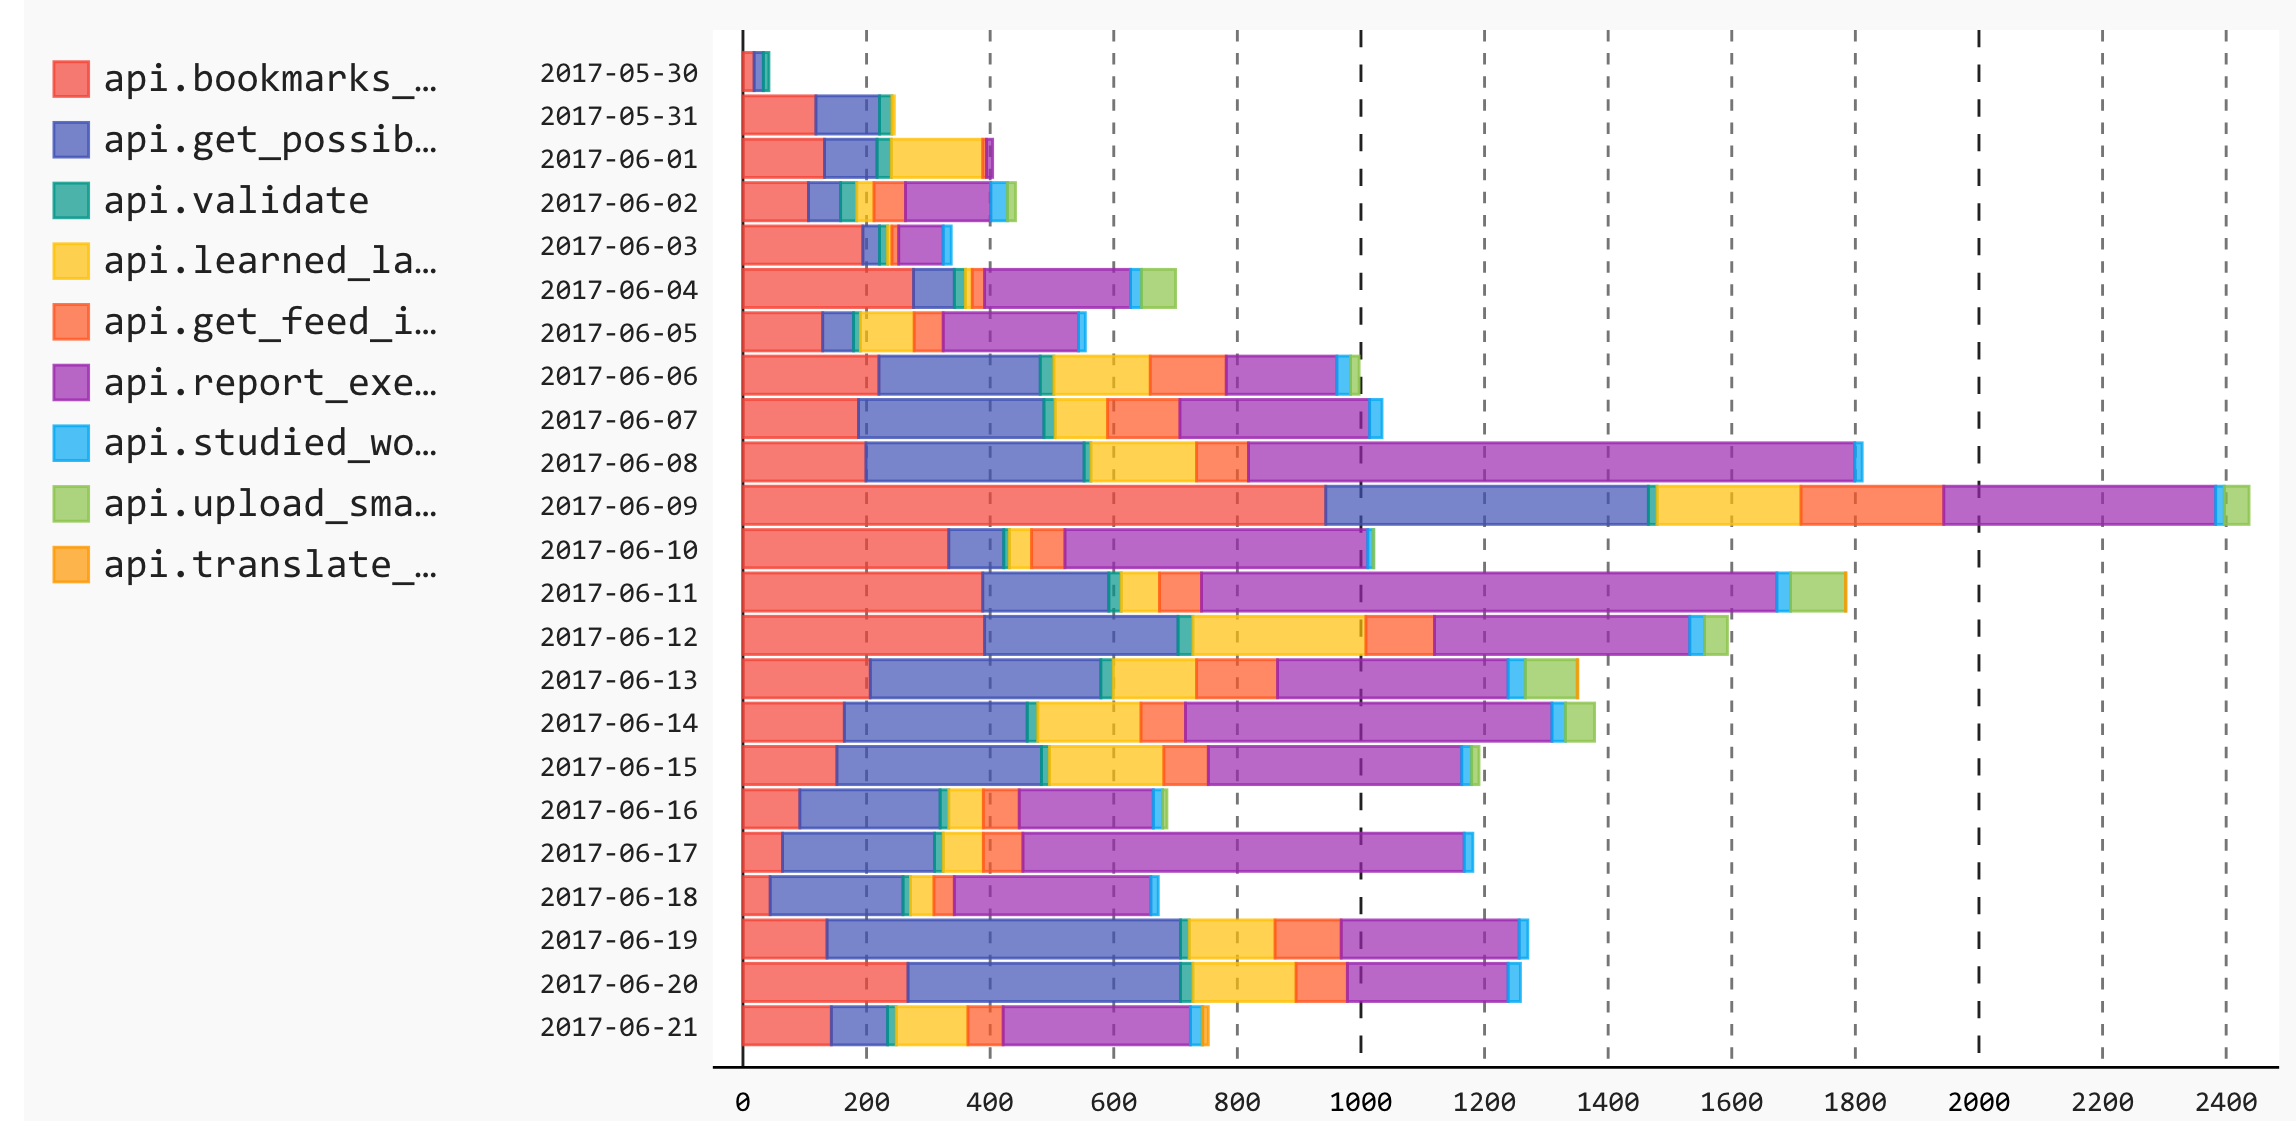
\includegraphics[width=\linewidth]{all_endpoints_usage.png}
    \caption{The number of requests per endpoint per day view shows the overall utilization of the monitored application}
    \label{fig:aeu}
  \end{figure}

  This visualization also provides feedback to the maintainer when deciding aboiut endpoint deprecation, the most elementary way of {\em understanding the needs of the downstream} \cite{Haen14a}. In our case study, the maintainer decided to not remove several endpoints once they saw that, contrary to their expectations, they were being used.\footnote{Usage information can also be used to increase the confidence of the maintainer that a given endpoint is not used, although it is not a proof.}

  \niceseparator

  A second type of {\em utilization} question that an API maintainer can answer by using the \tool regards cyclic patterns of usage during various times of day. 
  % \mlv{can we provide some support for this claim? a reference maybe?}

  % \mltp{ can we add vertical lines that highlight the beginng of a new week (e.g. before Sunday): }

    \begin{figure}[h!]
      \centering
      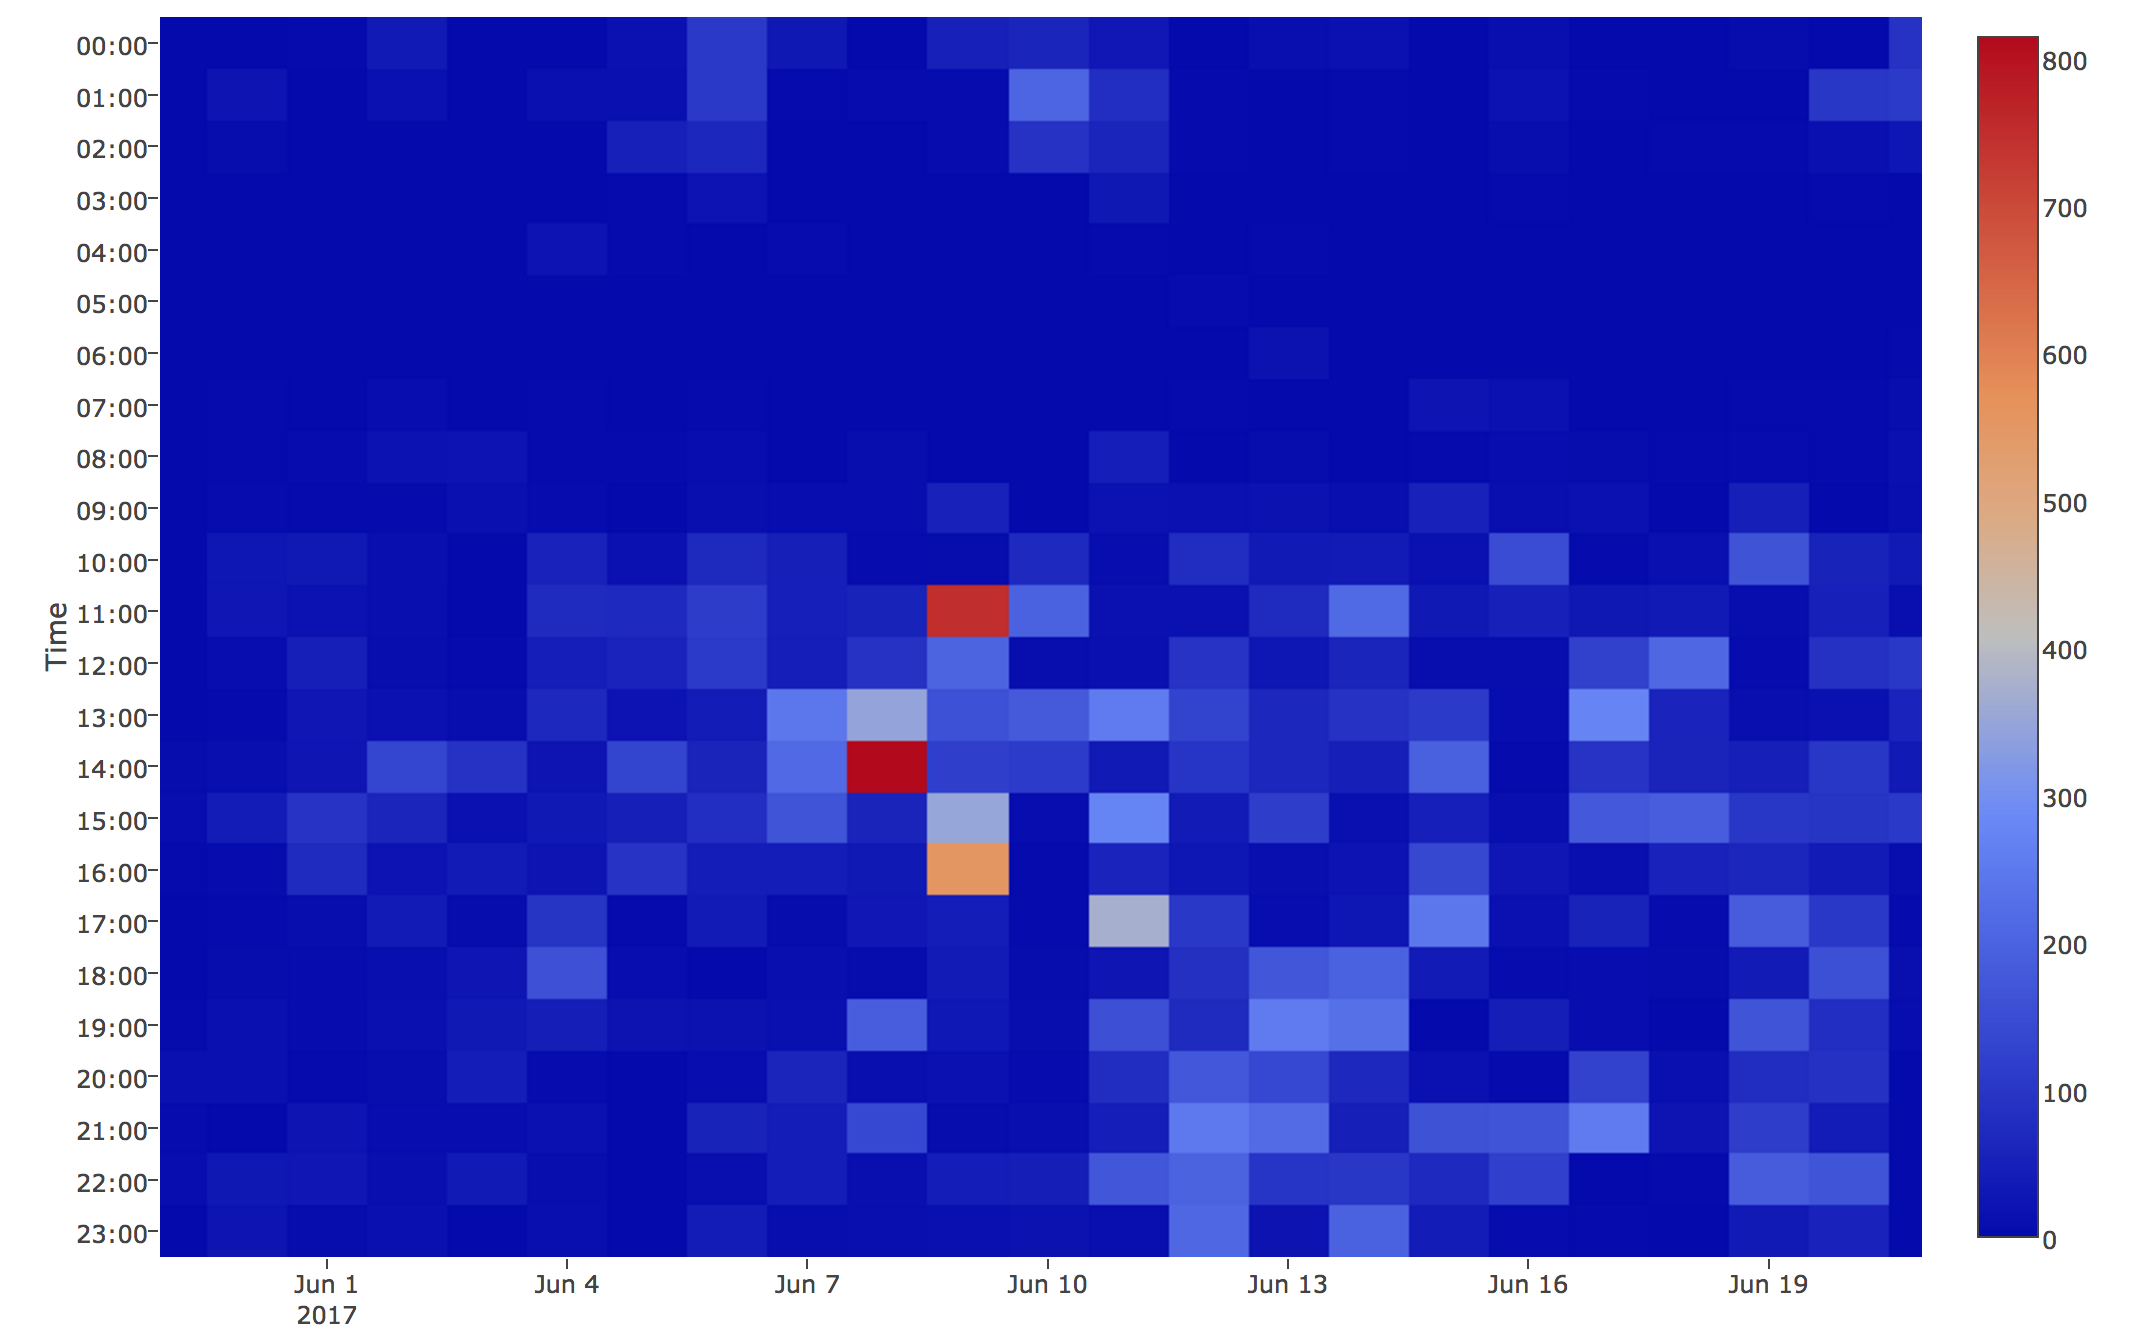
\includegraphics[width=\linewidth]{daily_patterns}
      \caption{Usage patterns become easy to spot in the requests per hour heatmap}
      \label{fig:dp}
    \end{figure}


  Figure \ref{fig:dp} shows the users of the Zeeguu API not practicing  languages at night, but otherwise hitting the API around the clock with several hundred hits per hour. 


\newpage
\section{Visualizing Service Performance}

  The \tool also collects information regarding endpoint performance. The view in Figure \ref{fig:ep} summarizes the response times for various endpoints by using boxplots. 

  % \ml{Thijs and Patrick... the visualization people will complain when they see that we have different colors for the same endpoint in different graphs. Can we insure that there is consistency in colors? Simplest trick would be to obtain the color by hashing the name of the endpoint... in that case the same endpoint woudl have the same color in various graphs.}

  \begin{figure}[h!]
    \centering
    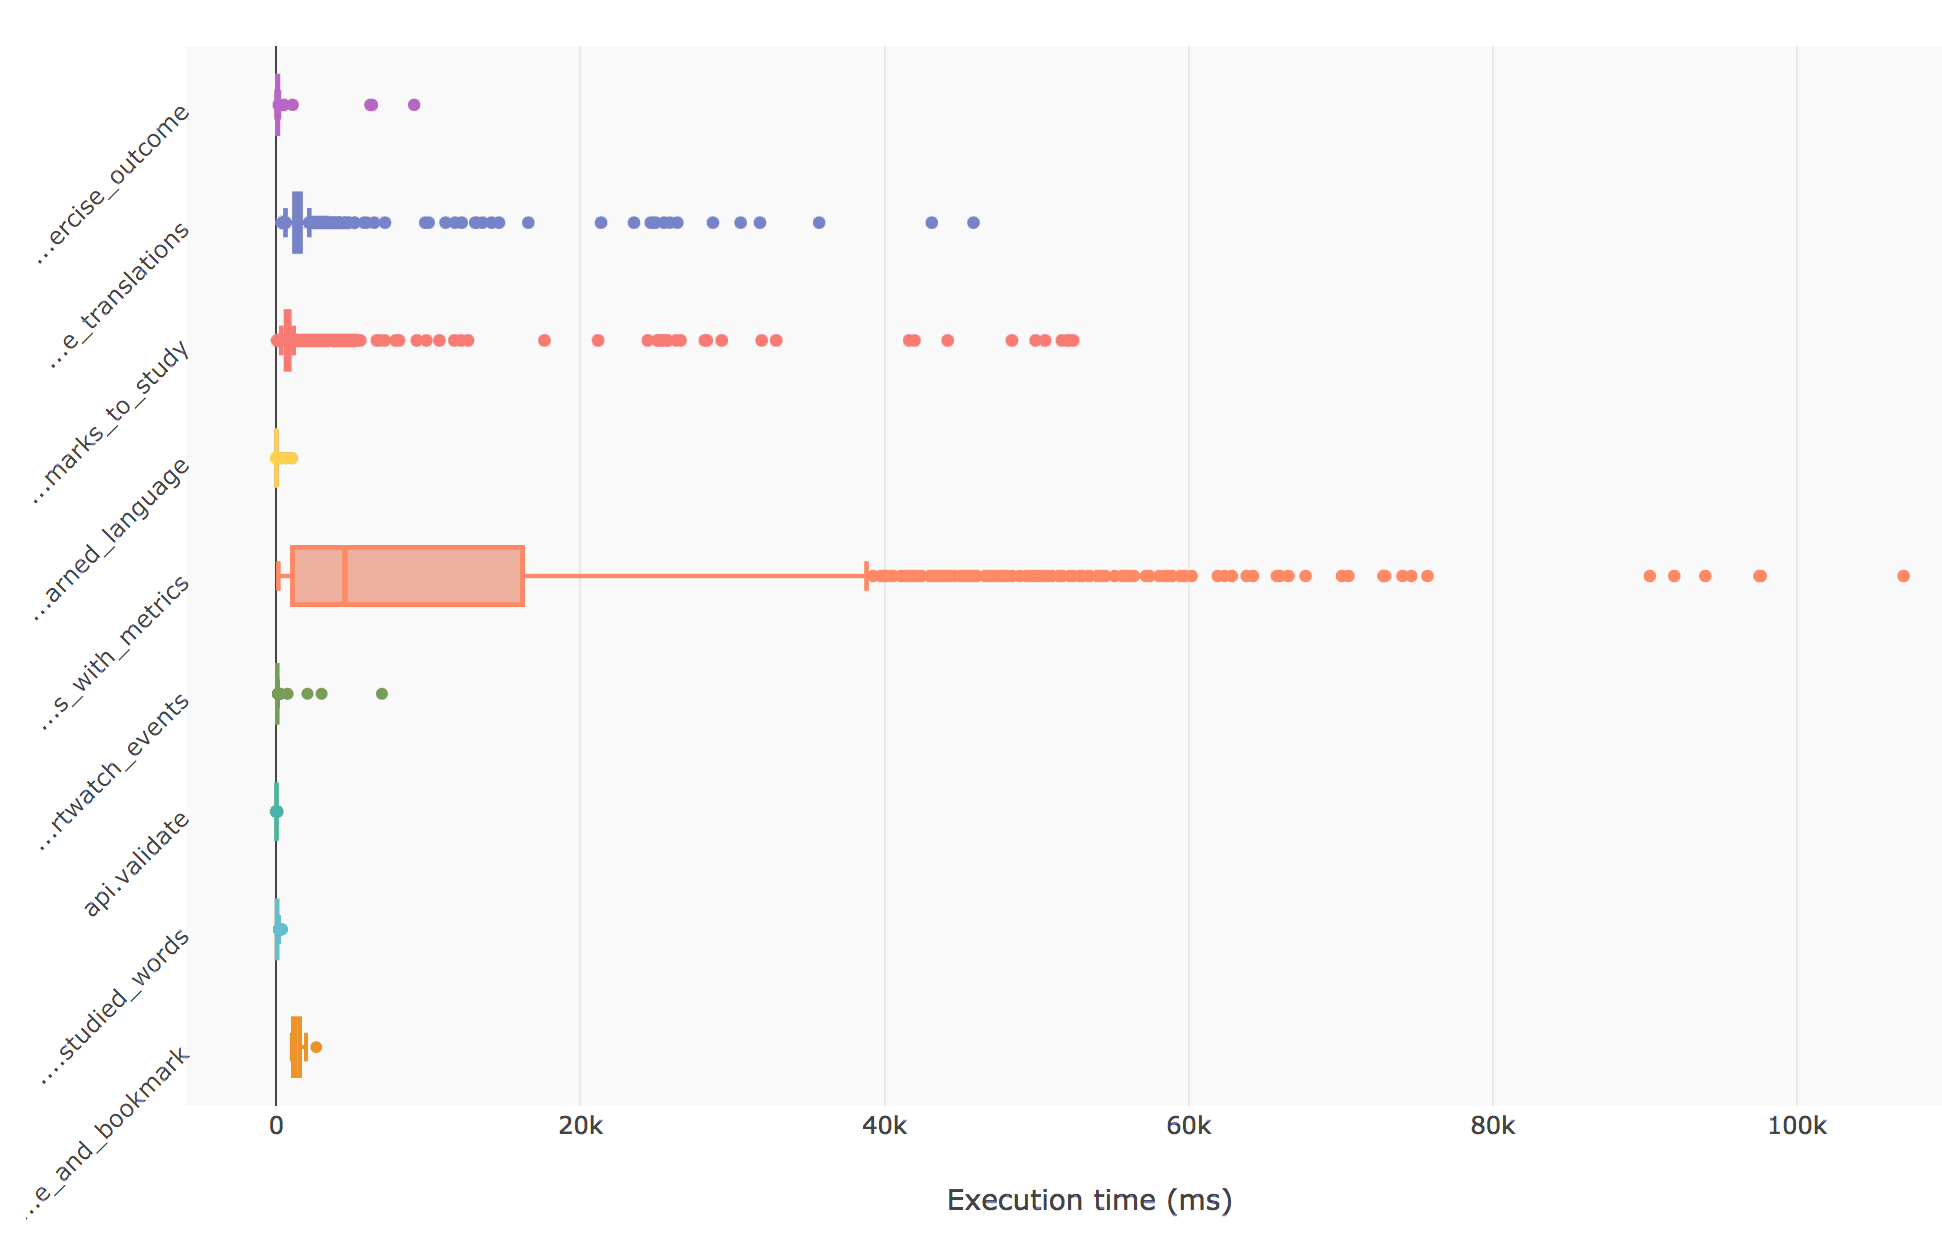
\includegraphics[width=\linewidth]{endpoint_performance.png}
    \caption{The response time (in ms) per monitored endpoint view allows for identifying performance variability and balancing issues}
    \label{fig:ep}
  \end{figure}

  After investigating this view it became clear to the maintainer that three of the endpoints had very large variation in performance. One of the three was most critical was optimized first: the \epTranslations is part of a live interaction and it having such variable performance was a usability problem for the users of the reader applications. 

  % most important endpoints that they decided to improve the performance of is the second from the top in Figure \ref{fig:ep}: the endpoint that returns translations. This is particularily critical since it is part of a live interaction loop. 

\newpage
  \niceseparator

  To be able to see their improvements in action, the maintainer had to add an extra configuration information to be able to find the `.git' folder from where to retrieve the current version of the deployed application: 

  \begin{lstlisting}[caption=Configuring the \tool with the path to the .git folder enables the generation of evolutionary performance graphs, style=custompython]

  dashboard.config.git = 'path/to/git-root/of/app'

  \end{lstlisting}

  After redeploying the API, the dashboard can now automatically detect the current version of the project, and can group measurements by version. \tool can now generate the view in Figure \ref{fig:tee} where the performance of the give endpoint is tallied by version.

  \begin{figure}[h!]
    \centering
    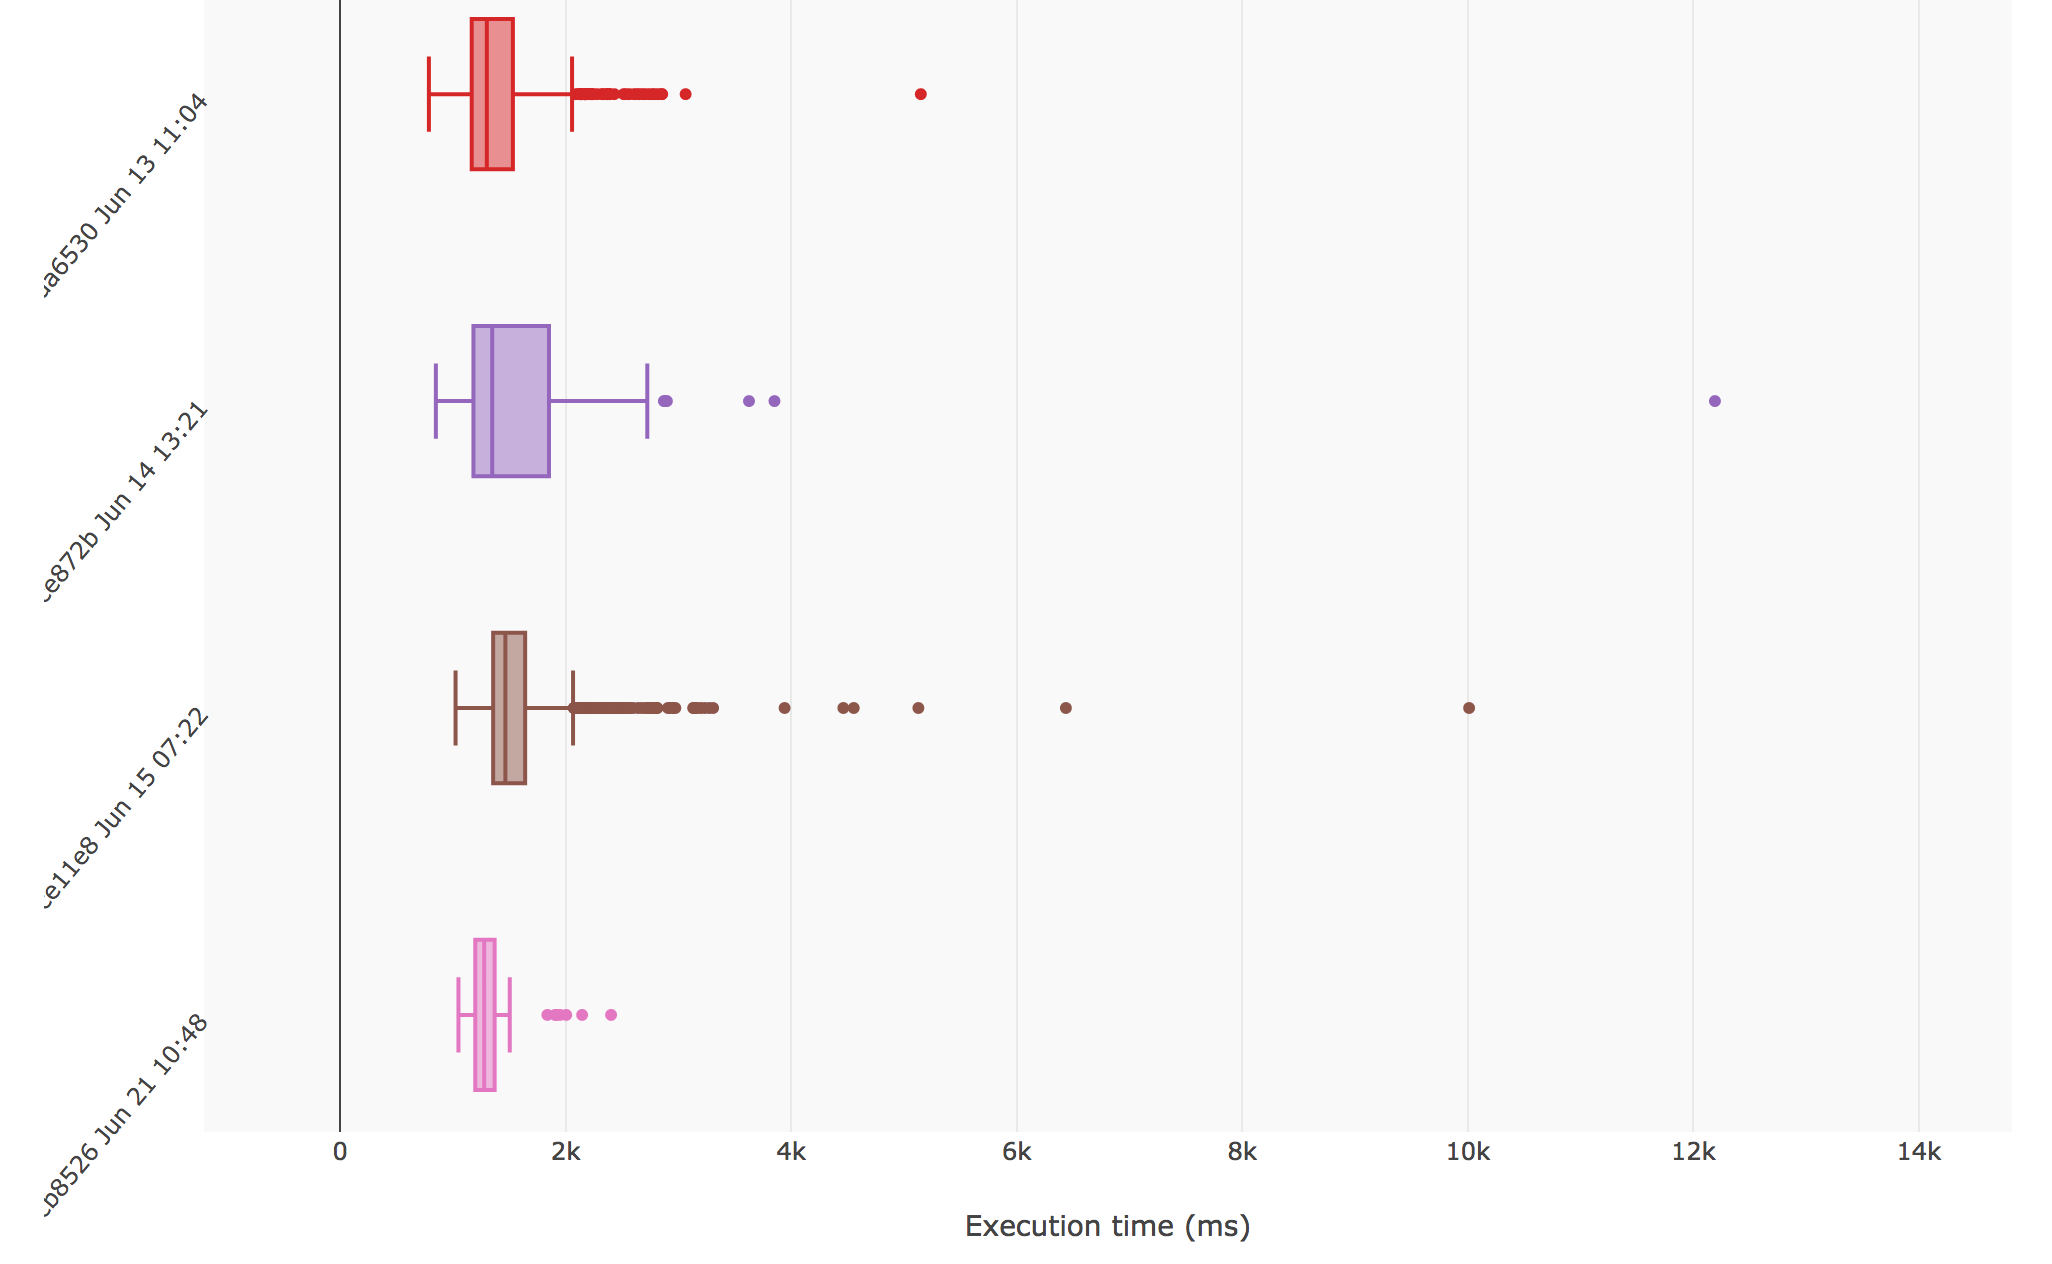
\includegraphics[width=\linewidth]{translation_endpoint_evolution.png}
    \caption{Visualizing The Performance Evolution of the \epTranslations endpoint}
    \label{fig:tee}
  \end{figure}

  This way the maintainer could confirm that the performance of the translation endpoint improved: in the latest version (bottom-most box plot in Figure \ref{fig:tee}) the entire boxplot moved to the left and there are fewer outliers.


  \niceseparator

  The \tool also collects {\bf extra informaiton about outliers}: Python stack trace, CPU load, request parameters, etc. in order to allow the maintainer to investigate the causes of these exceptionally slow response times. 

  In order to address this, but not degrade the usual performance the \tool tracks for every endpoint a running average value. When it detects that a given request is an outlier with respect to this past average running value, it triggers the {\em outlier data collection routine} which stores all the previously listed extra information about the current execution environment. 


\section {User Centered Visualization}

  For service endpoints which run computations in real time as they are called, there might be very different timings based on the different loads that are sent to the endpoint. 

  In our cases study, one of the slowest endpoints, and one with the higest variability is \epFeedItems: it retrieves a list of recommended articles for a given user. However, since a user can be subscribed to anything from one to three dozen article sources, and since the computation of the difficulty is personalized and it is slow, the variability in time among users is likely to be very large. 

  \tool provides a way of grouping information on a per user basis. However, to do this, the developer must specify the way in which a given API call can be associated with a given user. There are multiple ways, the simplest takes again advantage of the strengths of the Flask framework which offers a global request object which contains session information: 

  \begin{lstlisting}[float,caption=TBA,style=custompython]
    
    # app specific way of extracting the user
    # from a flask request object    
    def get_user_id(request):
      sid = int(request.args['session'])
      session = User.find_for_session(sid)
      return user_id

    # attaching the get_user_id function
    dashboard.config.get_group_by = get_user_id

  \end{lstlisting}


  Sometimes, grouping the service calls per endpoint it is not sufficient. Figure \ref{fig:tpu} shows some of the results of calling the \epFeedItems endpoint for various users. 

  \begin{figure}[h!]
    \centering
    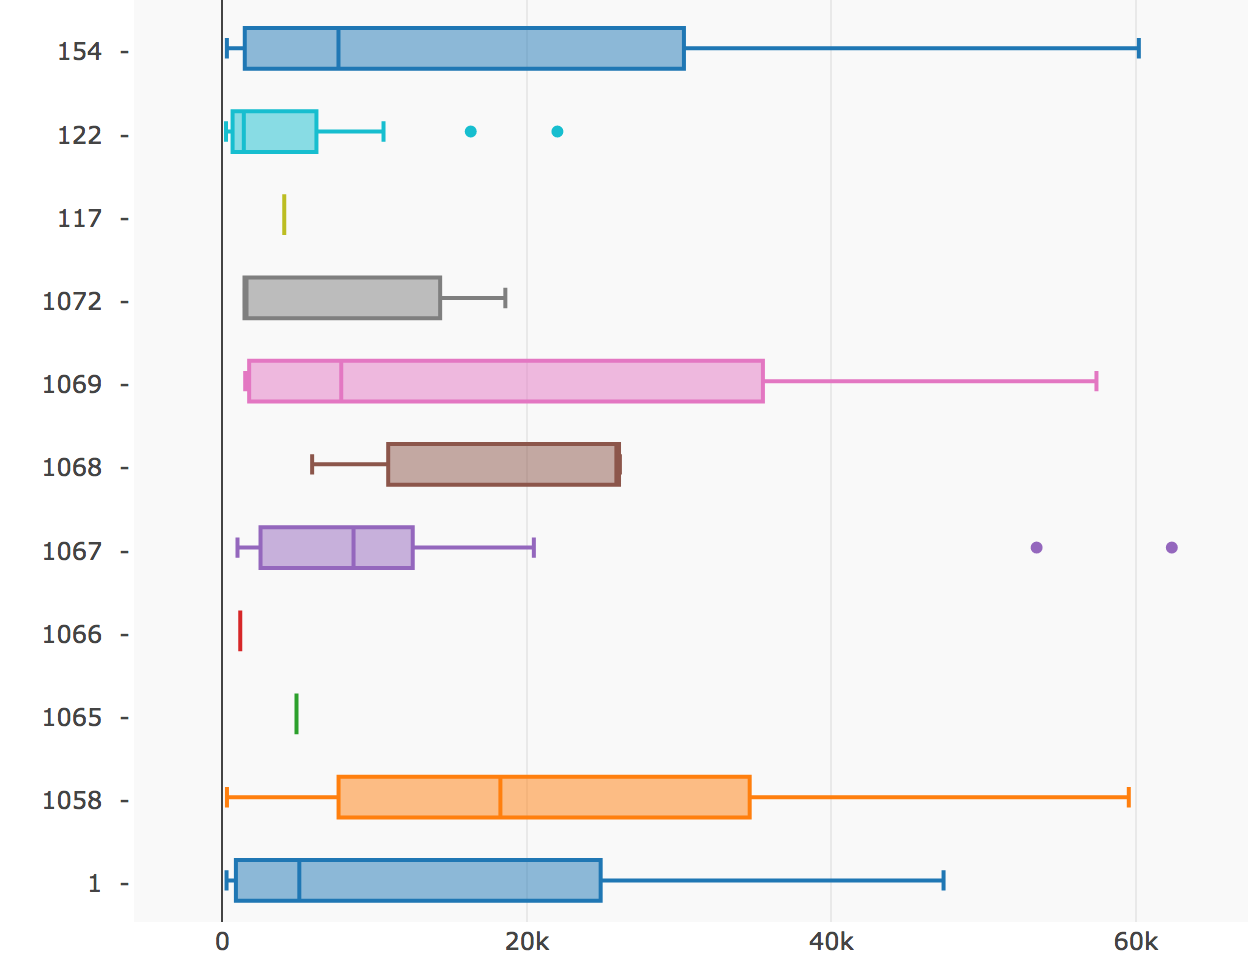
\includegraphics[width=\linewidth]{time_per_user}
    \caption{The \epFeedItems shows a very high variability across users}
    \label{fig:tpu}
  \end{figure}


  Different users might have different experiences: 
  - a user has 10K emails one has 10 emails
  - a user is subscribed to 20 feeds one to 2 feeds

  The system will have different processing times. 
  It is important for the DevOps-er to be able to understand the difference in performance on a per user basis. 

  If we try to show also per version: 

  \begin{figure}[h!]
    \centering
    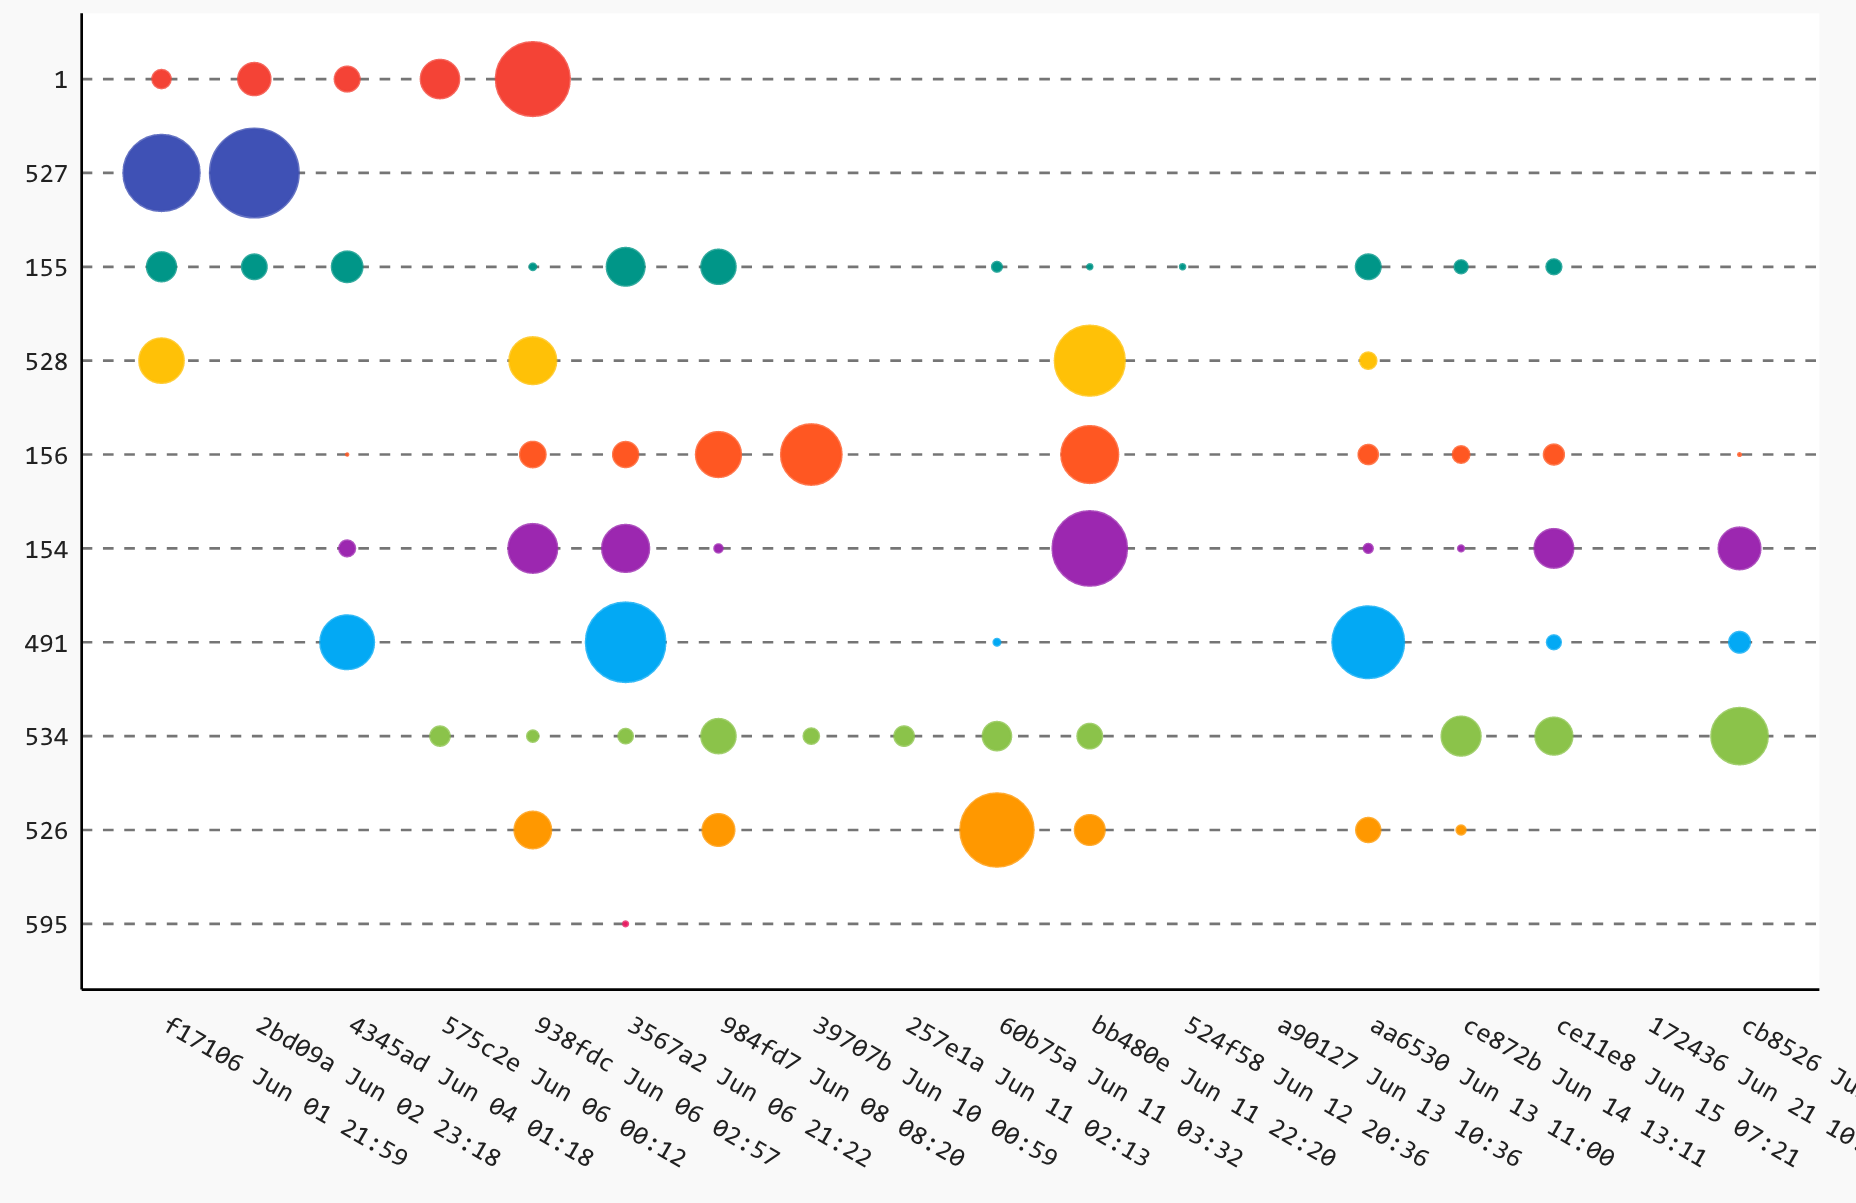
\includegraphics[width=\linewidth]{time_per_user_per_version}
    \caption{Caption here}
    \label{fig:figure1}
  \end{figure}



\section{Tool Availability}

The code of \tool is available under an open-source permissive MIT license on Github \footnote{\url{https://github.com/mircealungu/automatic-monitoring-dasboard}}.

The images in this paper are screenshots of the actual deployment of the tool which can be found at {https://zeeguu.unibe.ch/api/dashboard}. For the readers of this paper to be able to see the tool in action, they can login with the username and password: guest, dashboardguest!. 
\mltp{we should add a guest/guest username password which is allowed to only visualize things, but not modify anything, and not export anything!}

\section{Related Work}

Java Visualization \cite{Pauw02a}

Run-time monitoring of services \cite{ghezzi2007run}

\section{Conclusion}
The conclusion goes here.




% conference papers do not normally have an appendix


% use section* for acknowledgment
\section*{Acknowledgment}


The authors would like to thank...





% references section

\bibliographystyle{IEEEtran}
\bibliography{vissoft}


% that's all folks
\end{document}


